\documentclass{report}
\usepackage[utf8]{inputenc}
\usepackage[spanish]{babel}
\usepackage[margin=2cm]{geometry}
\usepackage{graphicx}
\usepackage{float}
\usepackage{titlesec}
\usepackage{caption}
\usepackage{listings}
\usepackage{xcolor}
\usepackage{array}
\usepackage{booktabs}
\usepackage{tabularx}
\usepackage{multirow}
\usepackage{amsmath}
\usepackage{hyperref}

\definecolor{codegreen}{rgb}{0,0.6,0}
\definecolor{codegray}{rgb}{0.5,0.5,0.5}
\definecolor{codepurple}{rgb}{0.58,0,0.82}
\definecolor{backcolor}{rgb}{0.95,0.95,0.95}


\lstset{
    basicstyle=\ttfamily,
    inputencoding=utf8,
    extendedchars=true,
    literate=%
    {á}{{\'a}}1
    {é}{{\'e}}1
    {í}{{\'i}}1
    {ó}{{\'o}}1
    {ú}{{\'u}}1
    {ñ}{{\~n}}1
    {Á}{{\'A}}1
    {É}{{\'E}}1
    {Í}{{\'I}}1
    {Ó}{{\'O}}1
    {Ú}{{\'U}}1
    {Ñ}{{\~N}}1
}


\lstdefinestyle{mystyle}{
    backgroundcolor=\color{backcolor},
    commentstyle=\color{codegreen},
    keywordstyle=\color{red},
    numberstyle=\tiny\color{codegray},
    stringstyle=\color{codepurple},
    basicstyle=\ttfamily\footnotesize,
    breakatwhitespace=false,
    breaklines=true,
    captionpos=b,
    keepspaces=true,
    numbers=left,
    showspaces=false,
    showstringspaces=false,
    showtabs=false,
    tabsize=2  
}

\titleformat{\section}
{\huge\bfseries}{\thesection.}{1em}{}
\titleformat{\subsection}
{\large\bfseries}{\thesubsection}{1em}{}

\renewcommand\thesection{\arabic{section}}

\title{\Huge{\textbf{Practica 4. Optimización por Enjambre de Particulas.}}\\
\Large{\textbf{Algoritmos Bioinspirados}}}
\author{Diego Castillo Reyes\\Marthon Leobardo Yañez Martinez\\Aldo Escamilla Resendiz}

\graphicspath{{imagenes/}}

\begin{document}
    \maketitle
    \tableofcontents
    \newpage
    \section{Introducción}
    La Optimización por Enjambre de Partículas (PSO por sus siglas en inglés, Particle Swarm Optimization) es una técnica de optimización inspirada en el comportamiento social de los animales, particularmente en el vuelo de las aves y el movimiento de los peces en bancos. Esta técnica se basa en un enfoque colaborativo, donde un conjunto de soluciones candidatas, representadas como "partículas", navegan a través de un espacio de búsqueda buscando la óptima global siguiendo reglas simples.

    Cada partícula en el enjambre ajusta su posición y velocidad de acuerdo con su propia experiencia pasada y la información compartida por las otras partículas. A medida que el algoritmo avanza en el tiempo, las partículas convergen gradualmente hacia las regiones de alta calidad del espacio de búsqueda, buscando mejorar el desempeño de la solución.

    El PSO ha demostrado ser efectivo en una amplia gama de problemas de optimización, incluyendo la optimización de funciones matemáticas, diseño de ingeniería, problemas de programación, entre otros. Su simplicidad conceptual y su capacidad para escapar de óptimos locales lo hacen una herramienta valiosa en la caja de herramientas de los investigadores y profesionales en campos como la ingeniería, la ciencia de datos y la inteligencia artificial.

    \section{Estadísticas Descriptivas}
    \begin{table}[H]
        \centering
        \begin{tabular}{|c|c|c|c|}
        \hline
        \multirow{2}{*}{Conf} & \multirow{2}{*}{Estadíst.} & \multicolumn{2}{c|}{Funciones de prueba} \\ \cline{3-4} 
                              &                             & Ackley & Rosenbrock \\ \hline
        1 (0.25,0.0,0.0)                    & min                         & 18.515644131362567 & 498.35182704181545 \\ \cline{2-4} 
                              & max                         &     21.95       &    1,084   \\ \cline{2-4} 
                              & promedio                    &      21.090003122849488      &    4553.570892237594    \\ \cline{2-4} 
                              & des. est.                   &   11.9414              &    195.9769        \\ \hline
        2 (0.25,0.0,1.0)                    & min                         &     9.517998536467005   & 16.59913616876128    \\ \cline{2-4}
                              & max                         &  22.02   &    1,093    \\ \cline{2-4}
                              & promedio                    &    9.517998536467003    &  16.59913616876128   \\ \cline{2-4}
                              & des. est.                   &   9.2297            & 18.6567        \\ \hline
        3 (0.25,0.0,2.0)                    & min                         &      4.976418408338478      &     10.667890800223562   \\ \cline{2-4} 
                              & max                         &     22.09       &     1,095   \\ \cline{2-4} 
                              & promedio                    &      4.9764184083384775      &    10.667890800223566    \\ \cline{2-4} 
                              & des. est.                   &   14.6730            &    12.3508        \\ \hline
        4 (0.25,1.0,0.0)                    & min                         &      18.515644131362567      &    498.35182704181545    \\ \cline{2-4} 
                              & max                         &     21.94       &   1,088     \\ \cline{2-4} 
                              & promedio                    &     21.090003122849488       &   4553.570892237594     \\ \cline{2-4} 
                              & des. est.                   &   196.8121            &   11.8948        \\ \hline
        5 (0.25,1.0,1.0)                    & min                         &    9.517998536467005        &   16.59913616876128     \\ \cline{2-4} 
                              & max                         &        21.85    &    1,088    \\ \cline{2-4} 
                              & promedio                    &      9.517998536467003      &     16.59913616876128   \\ \cline{2-4} 
                              & des. est.                   &       15.8619            &        4.9487        \\ \hline
        6 (0.25,1.0,2.0)                    & min                         &    4.976418408338478        &    10.667890800223562    \\ \cline{2-4} 
                              & max                         &        21.87    &     1,095   \\ \cline{2-4} 
                              & promedio                    &     4.9764184083384775       &   10.667890800223566     \\ \cline{2-4} 
                              & des. est.                   &   1.5339            & 6.2262       \\ \hline
        7 (0.25,2.0,0.0)                    & min                         &    18.515644131362567        &   498.35182704181545     \\ \cline{2-4} 
                              & max                         &        21.86    &     1,088   \\ \cline{2-4} 
                              & promedio                    &      21.090003122849488      &   4553.570892237594     \\ \cline{2-4} 
                              & des. est.                   &  193.8826          &  12.4578      \\ \hline
        8 (0.25,2.0,1.0)                    & min                         &      9.517998536467005      &    16.59913616876128    \\ \cline{2-4} 
                              & max                         &     21.96       &    1,085    \\ \cline{2-4} 
                              & promedio                    &     9.517998536467003       &   16.59913616876128     \\ \cline{2-4} 
                              & des. est.                   &   2.7139         &  13.7995      \\ \hline
        9 (0.25,2.0,2.0)                   & min                         &      4.976418408338478      &  10.667890800223562      \\ \cline{2-4} 
                              & max                         &      21.83      &   1,095     \\ \cline{2-4} 
                              & promedio                    &     4.9764184083384775       &    10.667890800223566    \\ \cline{2-4} 
                              & des. est.                   &    1.3678        &   1.1946     \\ \hline
        10 (0.5,0.0,0.0)                   & min                         &      0.1668246681319836      &     498.35182704181545   \\ \cline{2-4} 
                              & max                         &      22.09      &    1,085    \\ \cline{2-4} 
                              & promedio                    &      0.1668246681319836      &    4553.570892237594    \\ \cline{2-4} 
                              & des. est.                   &     11.9167       &   186.1457     \\ \hline

        \end{tabular}
        \caption{Resultados de las funciones de prueba}
        \label{tab:resultados}
    \end{table}

    \begin{table}[H]
        \centering
        \begin{tabular}{|c|c|c|c|}
        \hline
        \multirow{2}{*}{Conf} & \multirow{2}{*}{Estadíst.} & \multicolumn{2}{c|}{Funciones de prueba} \\ \cline{3-4}
                            &                             & Ackley & Rosenbrock \\ \hline

        11 (0.5,0.0,1.0)  & min                         &      2.031481808228964      &   9.861834458823816     \\ \cline{2-4} 
                              & max                         &     22.05       &   1,085     \\ \cline{2-4} 
                              & promedio                    &       2.031481808228964     &    9.86183445882382    \\ \cline{2-4} 
                              & des. est.                   &  8.4828          &  13.1460      \\ \hline
        12 (0.5,0.0,2.0)                   & min                         &     0.1668246681319836       &   8.778958901717523     \\ \cline{2-4} 
                              & max                         &       21.93     &   7,915     \\ \cline{2-4} 
                              & promedio                    &      0.1668246681319836      &     8.77895890171752    \\ \cline{2-4} 
                              & des. est.                   &    9.7346        &    1.6809    \\ \hline
        13 (0.5,1.0,0.0)                   & min                         &       18.515644131362567     &   498.35182704181545     \\ \cline{2-4} 
                              & max                         &     21.93       &   1,084     \\ \cline{2-4} 
                              & promedio                    &    21.090003122849488        &    4553.570892237594    \\ \cline{2-4} 
                              & des. est.                   &     13.1405       &  171.5325      \\ \hline
        14 (0.5,1.0,1.0)                   & min                         &      2.031481808228964      &  9.861834458823816      \\ \cline{2-4} 
                              & max                         &     22.0       &    1,081    \\ \cline{2-4} 
                              & promedio                    &     2.031481808228964       &    9.86183445882382    \\ \cline{2-4} 
                              & des. est.                   &  5.2824          &   9.5605     \\ \hline
        15 (0.5,1.0,2.0)                   & min                         &     0.1668246681319836       &   8.778958901717523     \\ \cline{2-4} 
                              & max                         &      21.96      &    7,915    \\ \cline{2-4} 
                              & promedio                    &      0.1668246681319836      &   8.77895890171752     \\ \cline{2-4} 
                              & des. est.                   &    5.0547        &  1.8957      \\ \hline
        16 (0.5,2.0,0.0)                   & min                         &      18.515644131362567      &    498.35182704181545    \\ \cline{2-4} 
                              & max                         &       21.95     &   1,081     \\ \cline{2-4} 
                              & promedio                    &     21.090003122849488       &   4553.570892237594     \\ \cline{2-4} 
                              & des. est.                   &    9.6494        &  146.7918      \\ \hline
        17 (0.5,2.0,1.0)                   & min                         &      2.031481808228964      &    9.861834458823816    \\ \cline{2-4} 
                              & max                         &       21.83     &    1,085    \\ \cline{2-4} 
                              & promedio                    &        2.031481808228964    &    9.86183445882382    \\ \cline{2-4} 
                              & des. est.                   &    1.6906        &  1.2368      \\ \hline
        18 (0.5,2.0,2.0)                   & min                         &     0.1668246681319836       &    8.778958901717523    \\ \cline{2-4} 
                              & max                         &      21.96      &     7,896   \\ \cline{2-4} 
                              & promedio                    &      0.1668246681319836      &    8.77895890171752    \\ \cline{2-4} 
                              & des. est.                   &   1.1079         & 1.3213       \\ \hline

        \end{tabular}
        \caption{Resultados de las funciones de prueba}
        \label{tab:resultados 2}
    \end{table}
    \section{Gráficas de convergencia}
    %inserta imagen Ackley.png
    \begin{figure}[H]
        \centering
        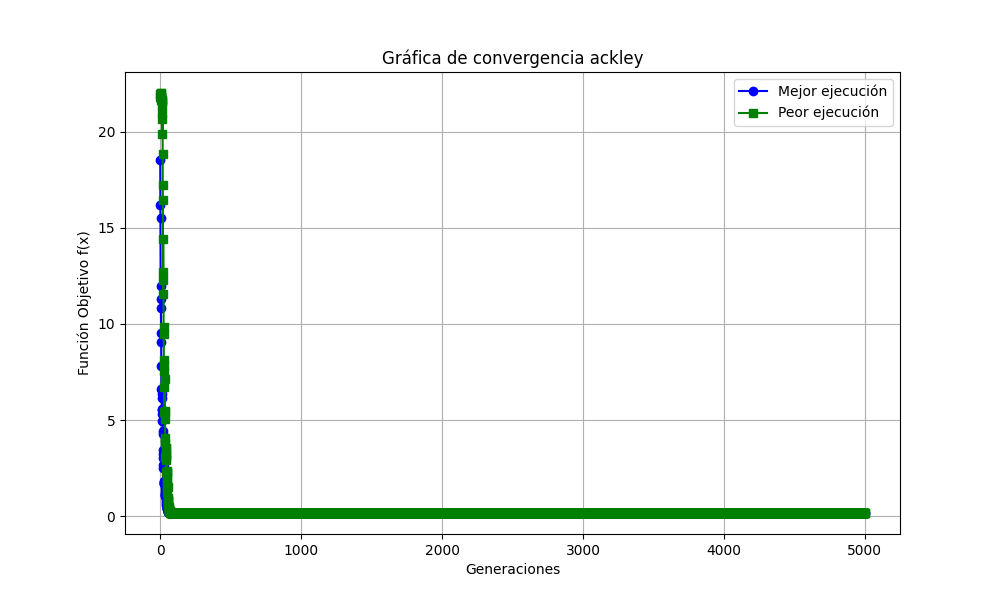
\includegraphics[width=0.8\textwidth]{Ackley.png}
        \caption{Convergencia de la función de Ackley}
        \label{fig:ackley}
    \end{figure}
    %inserta imagen Rosenbrock.png
    \begin{figure}[H]
        \centering
        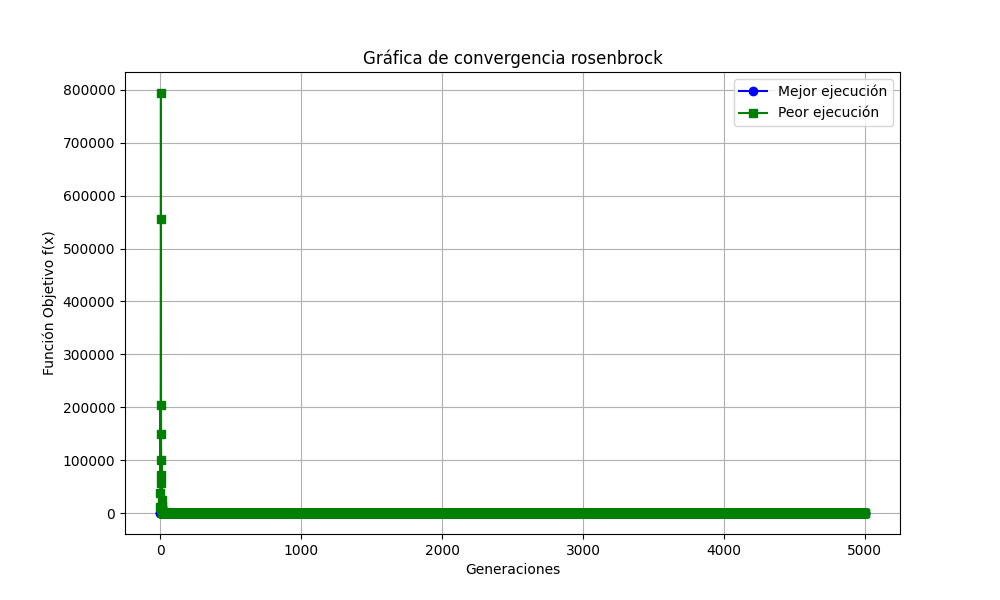
\includegraphics[width=0.8\textwidth]{Rosenbrock.png}
        \caption{Convergencia de la función de Rosenbrock}
        \label{fig:rosenbrock}
    \end{figure}
    %inserta imagen Rastrigin.png
    \begin{figure}[H]
        \centering
        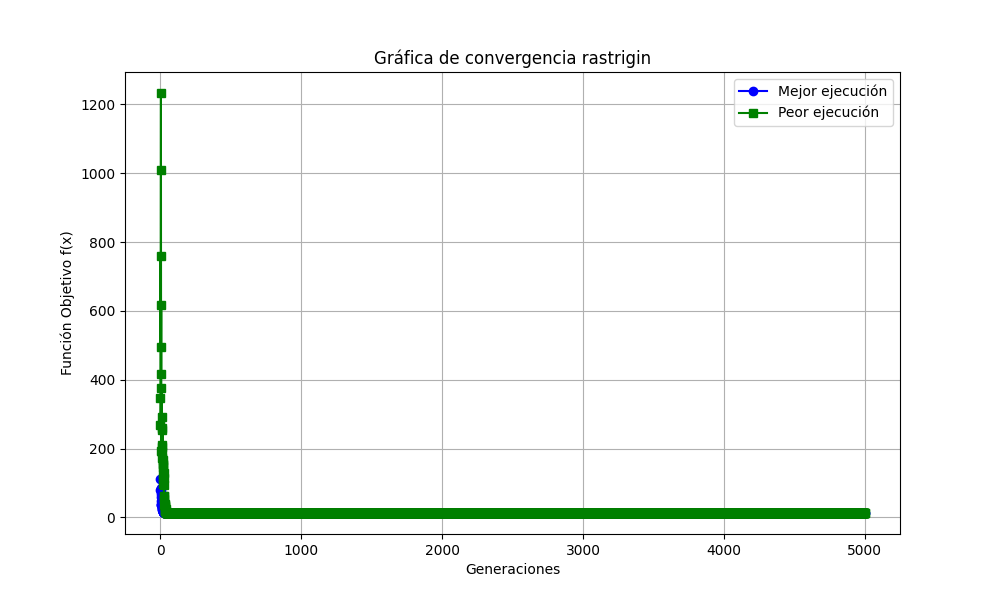
\includegraphics[width=0.8\textwidth]{rastrigin.png}
        \caption{Convergencia de la función de Rastrigin}
        \label{fig:rastrigin}
    \end{figure}
    %inserta imagen griewank.png
    \begin{figure}[H]
        \centering
        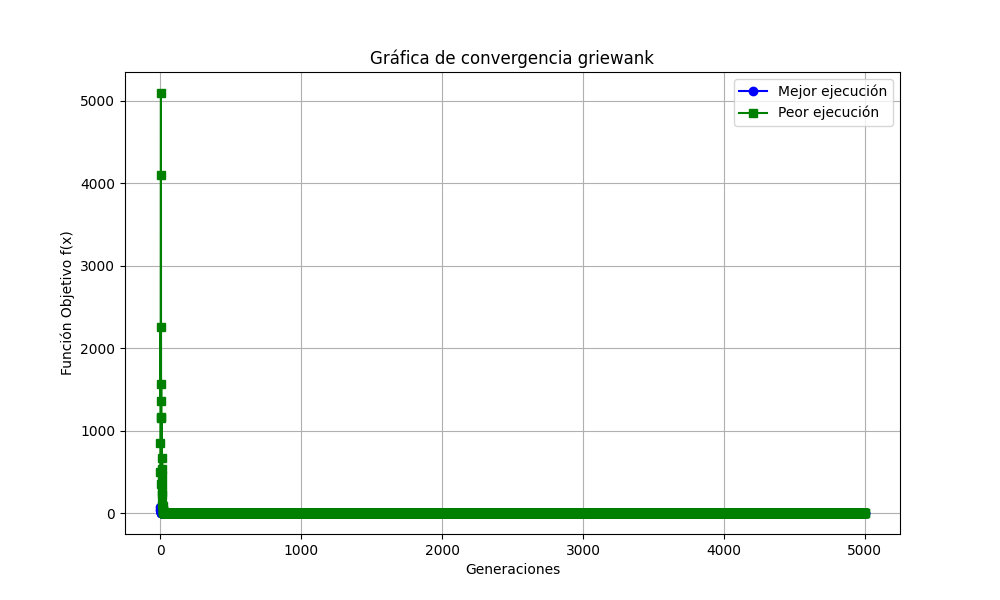
\includegraphics[width=0.8\textwidth]{griewank.png}
        \caption{Convergencia de la función de Griewank}
        \label{fig:griewank}
    \end{figure}
    \section{Análisis sobre el comportamiento del algoritmo de PSO}
    (a)  ¿Que efecto tiene aumentar los parámetros r1 y r2?\\
    Aumentar los parámetros r1 y r2 puede aumentar la diversidad de las partículas en el espacio de búsqueda, lo que puede ayudar a explorar nuevas regiones y evitar que las partículas se estanquen en óptimos locales. Sin embargo, un aumento excesivo en r1 y r2 puede llevar a una exploración excesiva y a una convergencia más lenta.\\
    (b)  En general, ¿a que valor de w le fue mejor?\\
    En general, el valor de w que mejor funcionó fue 0.25.\\
    (c)  ¿Cual es la peor configuración de parámetros para cada problema?\\
    La peor configuración de parámetros para el problema de Ackley es la configuración 10 (0.5,0.0,0.0) y para el problema de Rosenbrock es la configuración 10 (0.5,0.0,0.0).\\
    (d)  ¿Cual es el problema que converge mas rápido al optimo global y cual mas lento?\\
    El problema que converge mas rápido al optimo global es el problema de Ackley y el problema que converge mas lento es el problema de Rosenbrock.\\
    (e)  ¿Que mejoras realizaría en el algoritmo de PSO?\\ 
    Introducir mecanismos específicos para mejorar la convergencia, como estrategias de búsqueda local que se activan cuando las partículas se estancan, puede aumentar la eficiencia del PSO en la búsqueda de soluciones óptimas.  

    \section{Regresión lineal}
    \lstinputlisting[language=Python, style=mystyle]{psoRegresion.py}

    \section{Pruebas Realizadas}
    %inserta imagen PruebasRegresion.png
    \begin{figure}[H]
        \centering
        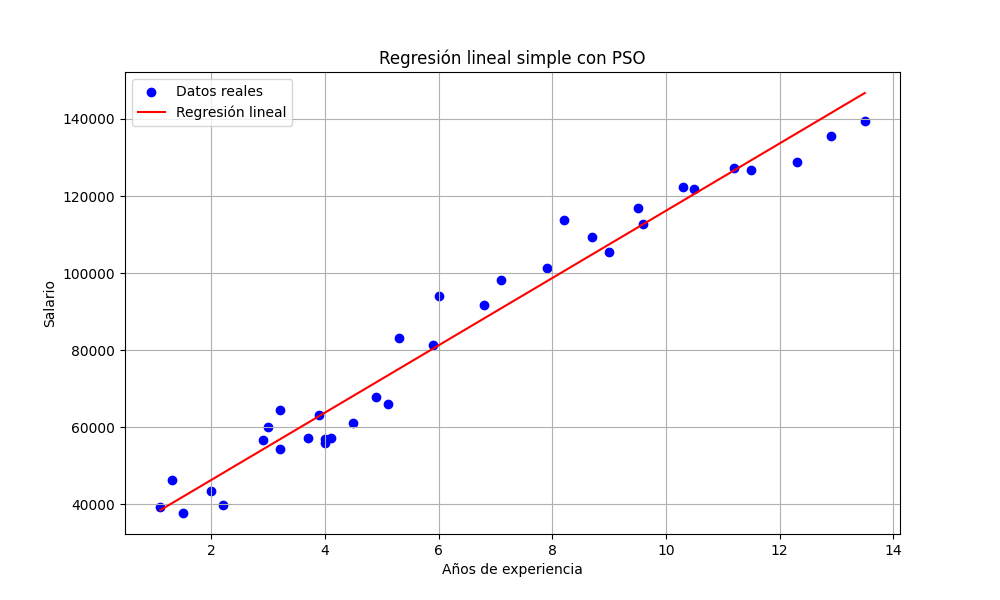
\includegraphics[width=0.8\textwidth]{PruebasRegresion.png}
        \caption{Pruebas de regresión}
        \label{fig:pruebas}
    \end{figure}
    \section{Lectura}
    En los últimos años, el número de enfoques de optimización bioinspirados ha crecido considerablemente, alcanzando niveles sin precedentes que ensombrecen las perspectivas 
    futuras de este campo de investigación. Este artículo aborda este problema proponiendo dos taxonomías exhaustivas y basadas en principios que permiten a los investigadores 
    organizar los desarrollos algorítmicos existentes y futuros en categorías bien definidas, considerando dos criterios diferentes: la fuente de inspiración y el comportamiento de cada algoritmo.\\ 
    Utilizando estas taxonomías, revisamos más de trescientas publicaciones sobre algoritmos bioinspirados y propuestas que caen dentro de cada una de estas categorías, llevando a un resumen crítico de las tendencias 
    de diseño y similitudes entre ellas, y la identificación del algoritmo clásico más similar para cada trabajo revisado. A partir de nuestro análisis, concluimos que a menudo se encuentra una relación pobre entre 
    la inspiración natural de un algoritmo y su comportamiento. Además, las similitudes en términos de comportamiento entre diferentes algoritmos son mayores de lo que se afirma en su divulgación pública: específicamente, 
    mostramos que más de un tercio de los solucionadores bioinspirados revisados son versiones de algoritmos clásicos. Basándonos en las conclusiones de nuestro análisis crítico, damos varias recomendaciones y puntos de mejora para mejores 
    prácticas metodológicas en este campo de investigación activo y en crecimiento.\\
    En los últimos años, se ha reportado una gran variedad de algoritmos bioinspirados en la literatura. 
    Estos algoritmos se utilizan en problemas de optimización complejos donde los solucionadores exactos no son aplicables debido a su coste computacional o tiempo de resolución. Inspirados en los procesos biológicos observados en la naturaleza, 
    estos algoritmos simulan procesos biológicos como la evolución natural y el comportamiento colectivo, dando lugar a conceptos como la \textit{Swarm Intelligence}.\\

    El artículo propone dos taxonomías principales:
    \begin{itemize}
    \item \textbf{Taxonomía basada en la fuente de inspiración:} Clasifica los algoritmos según su inspiración natural o biológica, permitiendo agrupar rápidamente los solucionadores publicados en la literatura.
    \item \textbf{Taxonomía basada en el comportamiento:} Clasifica los algoritmos según su comportamiento, es decir, cómo generan nuevas soluciones candidatas para la función a optimizar.
    \end{itemize}


    Del análisis de más de trescientas publicaciones, se concluye que existe una relación pobre entre la inspiración natural y el comportamiento del algoritmo. 
    Además, muchas soluciones bioinspiradas son variantes de algoritmos clásicos. Se proporcionan recomendaciones para mejorar las prácticas metodológicas en la investigación, 
    fomentando la aplicación de estos algoritmos a más problemas y la participación en competiciones para evaluar su rendimiento.\\


    El artículo destaca la necesidad de organizar los algoritmos bioinspirados en taxonomías claras para facilitar su análisis y comparación. Se enfatiza que el comportamiento del algoritmo es más relevante que su inspiración natural, 
    y se recomienda a los investigadores enfocarse en diferencias de comportamiento y evidencias de rendimiento verificables en problemas prácticos.\\


    \section{Conclusiones}
    Castillo Reyes Diego\\
    En esta practica pude comprobar el funcionamiento de el algoritmo PSO, el cual demostró una gran eficacia para poder resolver problemas de optimización, asi como se demostró en el ejemplo con una regresión lineal, y en las funciones de Rosenbrock fue impresionante ver como estos algoritmos convergían muy rápido gracias a su eficiencia anteriormente mencionada
    
    Escamilla Reséndiz Aldo.\\
    El algoritmo \textit{Particle Swarm Optimization} (PSO) es un ejemplo destacado de la \textit{Swarm Intelligence} y ha demostrado ser un enfoque efectivo y versátil para resolver problemas de optimización complejos. PSO simula el comportamiento social de los pájaros en busca de comida, permitiendo que las partículas (soluciones candidatas) en el espacio de búsqueda ajusten sus posiciones basándose en la experiencia personal y la de sus vecinos. Este enfoque ha inspirado muchos otros algoritmos y ha demostrado ser robusto en una amplia gama de aplicaciones.

    Las funciones de prueba como la función de Rosenbrock y la función de Ackley son cruciales para evaluar y comparar el rendimiento de los algoritmos de optimización. La función de Rosenbrock, también conocida como el "valle de Rosenbrock" o "banana function", es una función no convexa utilizada comúnmente como un problema de prueba para los algoritmos de optimización debido a su forma de valle estrecho que lleva a un mínimo global. Por otro lado, la función de Ackley es conocida por su paisaje multimodal con muchos mínimos locales, lo que la hace particularmente desafiante y útil para probar la capacidad de los algoritmos para escapar de los óptimos locales.

    Yañez Martinez Marthon Leobardo\\
    En esta práctica se implementó el algoritmo PSO para resolver problemas de optimización en dos funciones de prueba: la funciones de Rosenbrock y un problema de regresión lineal
    El PSO es un algoritmo bioinspirado que simula el comportamiento social de las aves
    y los peces en busca de comida. Cada partícula en el enjambre ajusta su posición y velocidad de acuerdo con su propia experiencia pasada y la información compartida por las otras partículas. A medida que el algoritmo avanza en el tiempo, las partículas convergen gradualmente hacia las regiones de alta calidad del espacio de búsqueda, buscando mejorar el desempeño de la solución.
    En este caso el PSO ha demostrado ser increíblemente eficiente, lo cual nos demuestra una vez mas la importancia y el poder de estos algoritmos.

\end{document}